\documentclass[11pt,a4paper]{article}

\usepackage[T1]{fontenc}
\usepackage[utf8]{inputenc}
\usepackage{lmodern}
\usepackage{microtype}
\usepackage[margin=2.3cm]{geometry}
\usepackage{amsmath,amssymb}
\usepackage{booktabs}
\usepackage{graphicx}
\usepackage{caption}
\usepackage{float}
\usepackage[section]{placeins}
\usepackage{setspace}
\usepackage[authoryear,round]{natbib}
\usepackage[colorlinks=true,linkcolor=black,citecolor=black,urlcolor=blue]{hyperref}

\makeatletter
\setlength{\@fptop}{0pt}   % float-only pages start at the top
\makeatother
\captionsetup{font=small,labelfont=bf}
\setstretch{1.06}
\newcommand{\tabfit}[1]{\resizebox{\textwidth}{!}{\input{#1}}}

\title{\textbf{Time-Series Momentum in a Ten-ETF Universe:\\
Volatility Targeting, Regime-Conditioned Exposure and Crisis Performance, 2008 to 2026}}
\author{Zack Higham\\[2pt]
\small BSc Mathematics (Statistics, Financial and AI pathway), Queen Mary University of London}
\date{October 2026}

\begin{document}
\maketitle

\begin{abstract}
\noindent
This paper implements the time-series momentum (TSMOM) strategy of \citet{moskowitz2012} on ten liquid exchange-traded funds spanning equities, government bonds, commodities and currencies, over 222 months from April 2008 to September 2026. It separates performance into three layers: the trend signal, volatility targeting and a walk-forward regime overlay. Every design parameter was committed to version control before any result was computed. Volatility targeting raises the net Sharpe ratio from 0.26 to 0.45 and turns monthly skewness from $-0.50$ to $+0.33$, but the gain is not statistically significant (bootstrap $p = 0.19$). The strategy gained 9.2\%, 12.6\% and 30.6\% in the three largest equity drawdowns of the sample and is highly correlated with the AQR futures TSMOM factor ($R^2 = 0.60$). The regime overlay lowers the Sharpe ratio to 0.39 and still trails when its average exposure is held at the unconditioned level; full-sample smoothed probabilities would have shown a spurious gain of 0.12. Deflated for the 26 configurations examined, the primary Sharpe ratio is not significant at 5\%. A pre-specified 20\% allocation beside a 60/40 portfolio cut the maximum drawdown from 32.3\% to 25.3\% and the loss in all six equity crisis windows; its Sharpe gain, from 0.74 to 0.86, is not significant ($p = 0.08$). The evidence supports trend following as a crisis diversifier, not as a reliably profitable stand-alone strategy.
\end{abstract}

\section{Introduction}

Time-series momentum is the tendency of an asset's own past return to predict its future return. \citet{moskowitz2012} (MOP) document it across 58 futures contracts from 1985 to 2009: a portfolio that is long each contract whose trailing twelve-month excess return is positive and short each contract whose return is negative earns a large and persistent premium, with its strongest returns in extreme market moves. \citet{hurst2017} extend the evidence back over a century. Trend following of this kind is the core business of managed-futures funds, and its central selling point is ``crisis alpha'': positive returns during prolonged equity sell-offs, when diversification is most valuable \citep{fung2001}.

Two refinements are standard in practice. Volatility targeting scales positions inversely to their ex-ante volatility and the whole portfolio to a constant volatility target; \citet{kim2016} argue that much of the TSMOM premium is in fact a volatility-scaling effect. Regime conditioning varies exposure with an estimated market state \citep{hamilton1989,ang2002}, on the premise that trend strategies earn their returns in persistent ``trending'' regimes and lose in choppy ones.

This paper asks four questions about a TSMOM strategy built only from liquid ETFs over 2008 to 2026, a period widely regarded as difficult for trend followers. Does the strategy earn a positive risk-adjusted return? How much of its performance comes from the signal, from volatility targeting, and from a regime overlay? Does it deliver crisis alpha in the sample's equity drawdowns? And how robust is any of this to implementation choices, costs and multiple testing?

The design is deliberately conservative. Every parameter (universe, sample, signal horizon, volatility estimator, risk allocation, cost assumption and regime model) was fixed in a configuration file and committed to version control before the first backtest was run, so the repository history documents that nothing was tuned to the results. The primary results are reported for these settings; alternatives appear only as labelled robustness checks. Where a decision had to be made after results were seen, it is identified as such.

The main findings are as follows. Volatility targeting is the layer that matters: it raises the Sharpe ratio from 0.26 to 0.45 and turns negative skewness positive, although the gain is not statistically significant. The volatility-targeted strategy gained in each of the three largest equity drawdowns, tracks the AQR futures TSMOM factor closely, and held at 20\% beside a 60/40 portfolio it lowered the maximum drawdown and the loss in every crisis window. The regime overlay adds nothing out of sample, and a smoothed-probability version shows how easily a lookahead error would have suggested otherwise. Once the number of configurations examined is taken into account, the primary Sharpe ratio is not distinguishable from what selection alone could produce.

\section{Data}
\label{sec:data}

\textbf{Universe.} The universe is ten U.S.-listed ETFs in four asset classes: equities (SPY, S\&P 500; EFA, developed markets excluding North America; EEM, emerging markets), U.S.\ Treasuries (IEF, 7 to 10 years; TLT, 20 years and over), commodities (GLD, physical gold; DBC, a diversified commodity futures basket) and currencies (UUP, long the U.S.\ dollar against the DXY basket; FXY, long the yen; FXA, long the Australian dollar). The currency sleeve uses three differentiated exposures: the broad dollar, a safe-haven currency and a commodity-linked currency. A euro fund was rejected because the euro is about 58\% of the dollar index, making it close to a duplicate of UUP (daily correlation $-0.95$). Short-duration Treasuries were excluded because their volatility of about 1.5\% would require extreme leverage under volatility targeting, and single-commodity funds were excluded as redundant with DBC and GLD.

\textbf{Prices.} Daily total-return prices and every distribution and split were downloaded from Yahoo Finance from 2 January 2002 to 30 September 2026. Rebuilding total returns from closing prices and distributions reproduces the adjusted series to within 6 basis points a year, the panel has no interior gaps, and every daily move larger than 8\% (49 in all) was matched to an identifiable market event.

\textbf{Risk-free rate and excess returns.} ETFs are fully funded, whereas the futures used in the TSMOM literature earn excess returns. Every return in this paper (in signals, volatility estimates and profit and loss) is therefore an excess return over the 13-week Treasury bill rate (Yahoo Finance \texttt{\^{}IRX}), accrued daily on an actual/360 basis from the yield known at the previous close; compounded to months, it has a correlation of 0.991 with the Kenneth French one-month bill series. This matters: in 2023 and 2024 cash earned about 5\% a year, and without it both the signals and the profit and loss of short positions would be misstated.

\textbf{Sample.} UUP begins trading in March 2007, so the first month-end at which all ten instruments have a twelve-month signal is 31 March 2008. The main sample is the 222 complete months from April 2008 to September 2026. Earlier data is used only for estimation warm-up and the regime model's training burn-in (Section~\ref{sec:regime_method}). The AQR Time Series Momentum factor, built from futures and forwards across the same four asset classes following MOP, is used as an external benchmark; it ends in May 2026, so comparisons with it cover 218 months.

Table~\ref{tab:data} summarises the instruments. SPY has the highest Sharpe ratio (0.72). The bond funds earned little in excess of cash (1.52\% a year for TLT and 1.12\% for IEF), because the 2022 sell-off reversed much of the earlier bond rally, and the yen lost 3.87\% a year against the dollar in excess-return terms. Table~\ref{tab:corr} reports monthly correlations. Within asset classes they are high (SPY and EFA 0.87, IEF and TLT 0.92), and the three currency funds are not independent (UUP and FXA $-0.78$). The effective number of independent bets within each class, measured by the eigenvalue participation ratio of its correlation matrix, is 1.26 for equities, 1.08 for rates, 1.87 for commodities and 1.93 for currencies. This motivates the risk allocation in Section~\ref{sec:vt}.

\begin{table}[!htbp]
\centering
\caption{Instruments, April 2008 to September 2026 (222 months). Annualised mean and volatility of monthly excess returns over the T-bill rate; the Sharpe ratio is their ratio. Skewness and worst month are for monthly returns.}
\label{tab:data}
\small
\begin{tabular}{llrrrrr}
\toprule
ETF & Class & Mean (\%) & Vol (\%) & Sharpe & Skew & Worst month (\%) \\
\midrule
SPY & Equity & 11.18 & 15.61 & 0.72 & $-$0.58 & $-$16.6 \\
EFA & Equity & 5.16 & 17.53 & 0.29 & $-$0.49 & $-$20.9 \\
EEM & Equity & 5.07 & 20.94 & 0.24 & $-$0.22 & $-$25.6 \\
IEF & Rates & 1.12 & 6.76 & 0.17 & 0.19 & $-$5.0 \\
TLT & Rates & 1.52 & 14.39 & 0.11 & 0.47 & $-$13.1 \\
GLD & Commodity & 7.91 & 17.44 & 0.45 & $-$0.04 & $-$16.2 \\
DBC & Commodity & 0.90 & 19.11 & 0.05 & $-$0.57 & $-$25.1 \\
UUP & FX & 1.26 & 7.79 & 0.16 & 0.17 & $-$6.4 \\
FXY & FX & $-$3.87 & 9.68 & $-$0.40 & 0.01 & $-$8.5 \\
FXA & FX & $-$0.57 & 12.40 & $-$0.05 & $-$0.24 & $-$15.5 \\
\bottomrule
\end{tabular}

\end{table}

\begin{table}[!htbp]
\centering
\caption{Correlations of monthly excess returns, April 2008 to September 2026.}
\label{tab:corr}
\small
\begin{tabular}{lrrrrrrrrrr}
\toprule
 & SPY & EFA & EEM & IEF & TLT & GLD & DBC & UUP & FXY & FXA \\
\midrule
SPY & 1.00 &  &  &  &  &  &  &  &  &  \\
EFA & 0.87 & 1.00 &  &  &  &  &  &  &  &  \\
EEM & 0.76 & 0.86 & 1.00 &  &  &  &  &  &  &  \\
IEF & $-$0.04 & 0.03 & 0.00 & 1.00 &  &  &  &  &  &  \\
TLT & $-$0.07 & $-$0.03 & $-$0.04 & 0.92 & 1.00 &  &  &  &  &  \\
GLD & 0.10 & 0.21 & 0.31 & 0.35 & 0.27 & 1.00 &  &  &  &  \\
DBC & 0.47 & 0.52 & 0.53 & $-$0.30 & $-$0.34 & 0.26 & 1.00 &  &  &  \\
UUP & $-$0.48 & $-$0.70 & $-$0.67 & $-$0.19 & $-$0.10 & $-$0.46 & $-$0.47 & 1.00 &  &  \\
FXY & $-$0.04 & 0.08 & 0.09 & 0.53 & 0.45 & 0.40 & $-$0.06 & $-$0.42 & 1.00 &  \\
FXA & 0.63 & 0.77 & 0.82 & 0.11 & 0.06 & 0.40 & 0.57 & $-$0.78 & 0.22 & 1.00 \\
\bottomrule
\end{tabular}

\end{table}

\section{Methodology}
\label{sec:method}

\subsection{Timing convention}

All signals and weights are computed from information available at the close of the last trading day of month $t$, and the resulting positions are held through month $t+1$. Trades execute at that same close, as in MOP; a one-day execution lag is reported as a robustness check. Between rebalances, positions drift with prices and the portfolio is marked to market daily, so that drawdowns inside a month (most importantly March 2020) are measured.

\subsection{Signals}

Let $r_{i,d}$ be the daily total return of instrument $i$ and $r^f_d$ the bill return. The $k$-month signal at month-end $t$ is the sign of the cumulative excess return over the preceding $k$ months,
\begin{equation}
s^{(k)}_{i,t} = \operatorname{sign}\!\left( \frac{P_{i,t}}{P_{i,t-k}} - \prod_{d \in (t-k,\,t]} \bigl(1 + r^f_d\bigr) \right),
\end{equation}
where $P_{i,t}$ is the total-return price at month-end $t$. The twelve-month signal is the primary specification, fixed in advance from MOP. Horizons of one, three and six months and an equal-weighted blend of the four signs are reported so that the choice can be judged, not so that the best one can be chosen. Following MOP, no month is skipped.

\subsection{Ex-ante volatility}

Volatility is the exponentially weighted estimator of MOP,
\begin{equation}
\sigma^2_{i,t} = 252 \sum_{j \ge 0} (1-\delta)\,\delta^{j} \bigl(x_{i,t-j} - \bar{x}_{i,t}\bigr)^2, \qquad \frac{\delta}{1-\delta} = 60,
\end{equation}
where $x_{i,d}$ is the daily excess return and $\bar{x}_{i,t}$ its exponentially weighted mean. The centre of mass is 60 trading days, at least 120 observations are required, and the estimate dated $t$ uses data up to and including the close of $t$. Portfolio risk uses these volatilities with the trailing 252-day correlation matrix of daily excess returns, $\Sigma_t = D_t C_t D_t$.

\subsection{Strategy variants}
\label{sec:vt}

\textbf{V1: raw TSMOM.} Equal notional per instrument, $w_{i,t} = s_{i,t}/N$ with $N = 10$, so gross exposure is one.

\textbf{V2a: inverse-volatility weighting.} Each instrument receives a share $b_i$ of a risk budget, and its position is scaled so that its stand-alone ex-ante volatility equals that share of the 10\% target $\sigma^* $:
\begin{equation}
w^{\mathrm{2a}}_{i,t} = s_{i,t}\, b_i\, \frac{\sigma^*}{\sigma_{i,t}}, \qquad b_i = \frac{1}{4\,n_{c(i)}},
\end{equation}
where $n_{c(i)}$ is the number of instruments in the asset class of $i$. The risk budget is thus split equally across the four asset classes and then equally within each class. Because instruments within a class are highly correlated (Section~\ref{sec:data}), equal risk per instrument (the MOP convention) would give the near-duplicate equity and Treasury funds a multiple of their diversification value. This allocation was revised from equal risk per instrument before any result was computed; the per-instrument version is reported in Appendix~\ref{app:trials}.

\textbf{V2: volatility targeting (primary).} V2a weights are rescaled so that the ex-ante volatility of the whole portfolio equals the target:
\begin{equation}
w^{\mathrm{2}}_{t} = \lambda_t\, w^{\mathrm{2a}}_{t}, \qquad \lambda_t = \frac{\sigma^*}{\sqrt{ w^{\mathrm{2a}\prime}_{t}\, \Sigma_t\, w^{\mathrm{2a}}_{t}}}.
\end{equation}
Leverage is not capped in the primary specification, mirroring the futures literature; caps are robustness checks. The budgets fix stand-alone volatility, not risk contribution, so V2 is an inverse-volatility portfolio rather than an equal-risk-contribution portfolio, and correlated same-sign positions take more than their nominal share of risk (Table~\ref{tab:riskshares}).

\textbf{Benchmarks.} Long-only risk parity (LO-RP) applies the V2 construction with every signal set to $+1$, so it isolates what TSMOM adds beyond holding the same risk-balanced, leveraged book long; \citet{huang2020} argue that much of the TSMOM premium is of this static kind. SPY and a monthly-rebalanced 60/40 portfolio of SPY and IEF are passive benchmarks, reported without costs.

\subsection{Regime-conditioned exposure}
\label{sec:regime_method}

\textbf{Observation series.} The regime model (R1) is fitted to the weekly cross-asset trend payoff, which measures directly whether trend following is currently being rewarded. On each day $d$, every instrument with a twelve-month signal contributes its unit-risk TSMOM return $s_{i,m(d)}\, x_{i,d} / \sigma_{i,m(d)}$, where $m(d)$ is the latest month-end strictly before $d$ (the position actually held on day $d$). The daily payoff is the average over the available instruments, and the weekly payoff $y_w$ is its sum over the week.

\textbf{Model.} The payoff follows a two-state Gaussian Markov-switching model \citep{hamilton1989} with state-dependent mean and variance,
\begin{equation}
y_w = \mu_{S_w} + \sigma_{S_w}\, \varepsilon_w, \qquad \varepsilon_w \sim \mathcal{N}(0,1), \qquad \Pr(S_w = j \mid S_{w-1} = i) = p_{ij},
\end{equation}
estimated by maximum likelihood with 20 random starting values, the best of which is kept.

\textbf{Walk-forward estimation.} At every month-end $t$ the model is re-estimated on all weeks ending on or before $t$, and the regime signal is the \emph{filtered} probability $\Pr(S_w = j \mid y_1, \ldots, y_w)$ of the last such week. Filtered probabilities use only past and current observations. Smoothed probabilities, $\Pr(S_w = j \mid y_1, \ldots, y_T)$, condition on the whole sample and are never used for any reported result. Because state labels are arbitrary in estimation, they are re-identified at every refit: the target (``trending'') state is the one with the higher mean payoff. At least 156 weeks are required. To have the overlay live for the 2008 crisis, the model is trained from 2003 on whichever instruments already have signals, so the number of instruments in the payoff rises from two (SPY and EFA) in 2003 to all ten by April 2008. A version trained on main-sample weeks only, and a version fitted to SPY returns instead of the trend payoff, are reported in Appendix~\ref{app:trials}.

\textbf{Overlay.} Variant 3 scales the V2 weights by an exposure multiplier,
\begin{equation}
w^{\mathrm{3}}_{t} = (0.5 + p_t)\, w^{\mathrm{2}}_{t},
\end{equation}
where $p_t$ is the target-state probability at $t$, so exposure varies between half and one and a half times V2. The portfolio is not re-targeted after the multiplier, which would cancel it.

\textbf{Lookahead illustration.} To quantify the bias that a common implementation error would create, the overlay is also computed from a single full-sample fit, using either its smoothed probabilities or its filtered probabilities. These variants use future data by construction; they are reported, clearly labelled, only as an illustration.

\subsection{Backtest engine and costs}

The backtest is a daily, self-financing simulation. With weights $w_{i,d-1}$ at the previous close, the portfolio's excess return on day $d$ is
\begin{equation}
R_d = \sum_i w_{i,d-1}\bigl(r_{i,d} - r^f_d\bigr) - c \sum_i \bigl| w^{\text{target}}_{i,d} - w_{i,d} \bigr| \mathbb{1}_{\text{trade}} - \text{fees}_d,
\end{equation}
and between trades the weights drift as $w_{i,d} = w_{i,d-1}(1 + r_{i,d})/(1 + r^f_d + R_d)$. Trading costs are $c = 10$ basis points per unit of notional traded, one way, with sensitivity from 0 to 50 basis points. This is conservative for these funds, whose quoted half-spreads are typically 1 to 5 basis points, but there is no market-impact model. Borrow fees on short positions and a financing spread over the bill rate on borrowed cash are sensitivity analyses. Monthly returns compound the daily excess returns: $\prod_d (1 + r^f_d + R_d) - \prod_d (1 + r^f_d)$.

\subsection{Statistical inference}

Means are tested with Newey-West $t$-statistics using the automatic lag rule of \citet{newey1994}, and Sharpe ratio standard errors follow \citet{lo2002}. Strategy variants built from the same signals are highly correlated, so Sharpe ratio differences are tested by resampling each pair of monthly return series jointly with the stationary bootstrap of \citet{politis1994} (mean block six months, 5,000 replications), in the spirit of \citet{ledoit2008}, with a two-sided $p$-value. Spanning regressions measure whether a strategy earns a return beyond a static combination of benchmarks. The volatility forecast is judged by the bias statistic, the standard deviation of monthly returns divided by their ex-ante monthly volatility, which equals one for a correct forecast. The deflated Sharpe ratio of \citet{bailey2014} adjusts the primary Sharpe ratio for the number of configurations examined and for non-normal returns.

\subsection{Validation of the implementation}

The code base has 42 automated tests. Those most relevant to bias are truncation tests: signals, volatilities, portfolio weights, backtest returns and walk-forward regime probabilities are recomputed after deleting all data after a cut-off date (including dates in the middle of the March 2020 crash), and every value dated before the cut-off is required to be unchanged. The engine is checked against hand-calculated cases, the targeted portfolio's ex-ante volatility against an independent covariance calculation, and the gross V1 returns against the textbook formula $N^{-1}\sum_i s_{i,t-1} r_{i,t}$, which they match exactly.

\section{Results}
\label{sec:results}

\subsection{Predictability at the instrument level}

Table~\ref{tab:predictive} reports pooled regressions of each instrument's volatility-scaled monthly excess return, $x_{i,t}/\sigma_{i,t-1}$, on its lagged signal, with standard errors clustered by month. The coefficients rise with the horizon, from $-0.001$ for the one-month signal to 0.016 for the twelve-month signal, the ordering found by MOP, but none is significant at 5\% (the twelve-month $t$-statistic is 1.66). With instrument fixed effects every $t$-statistic falls, to 1.02 for the twelve-month signal, because part of the pooled relation reflects differences in average returns across instruments rather than timing, the point made by \citet{huang2020}. MOP's lag-by-lag regressions show no more significant lags than chance would produce (Appendix Figure~\ref{fig:predictive}). A decomposition of the twelve-month sign strategy's average return into a timing component and a static component (the product of average position and average return) attributes 56\% to timing.

\begin{table}[!htbp]
\centering
\caption{Pooled predictive regressions of the volatility-scaled monthly excess return on the lagged $k$-month signal, 2,220 instrument-months. Standard errors clustered by month.}
\label{tab:predictive}
\small
\begin{tabular}{lrrrr}
\toprule
& \multicolumn{2}{c}{Pooled} & \multicolumn{2}{c}{Instrument fixed effects} \\
\cmidrule(lr){2-3}\cmidrule(lr){4-5}
Signal $s^k_{t-1}$ & Coef. & $t$ & Coef. & $t$ \\
\midrule
1m & $-$0.001 & $-$0.12 & $-$0.003 & $-$0.31 \\
3m & 0.014 & 1.36 & 0.010 & 0.93 \\
6m & 0.013 & 1.35 & 0.008 & 0.78 \\
12m & 0.016 & 1.66 & 0.010 & 1.02 \\
Blend & 0.019 & 1.31 & 0.012 & 0.74 \\
\bottomrule
\end{tabular}

\end{table}

Weak instrument-level predictability is consistent with a shorter, later and narrower sample than MOP's: 10 instruments rather than 58, over a period that includes the long, difficult stretch for trend followers in the 2010s. Whether a diversified, risk-managed portfolio earns a reliable return is a separate question, addressed next.

\subsection{The three layers of performance}

Table~\ref{tab:perf} reports performance net of costs, and Figure~\ref{fig:cumulative} the cumulative returns. The raw strategy V1 earns 1.79\% a year with 7.01\% volatility, a Sharpe ratio of 0.26 (Newey-West $t = 1.05$). Inverse-volatility weighting (V2a) raises the Sharpe ratio to 0.36 at much lower volatility, and targeting 10\% portfolio volatility (V2) raises it to 0.45, with an annual excess return of 5.07\% and a Newey-West $t$-statistic of 1.95. Volatility targeting also changes the shape of the return distribution: V1's monthly skewness is $-0.50$, V2's is $+0.33$, and at a quarterly horizon V2's skewness is $+0.82$. Positive skewness is a signature of trend following, and it appears here only after volatility scaling. V1's negative skewness comes largely from 2009, when its equal-notional book was short equities into the March 2009 rebound, a classic momentum crash \citep{daniel2016}.

\begin{table}[!htbp]
\centering
\caption{Performance, April 2008 to September 2026 (222 months). Trend strategies and LO-RP are net of 10 bps costs; SPY and 60/40 are gross. Mean and Vol: annualised excess return and volatility (\%). Sharpe with Lo (2002) standard error. NW $t$: Newey-West $t$-statistic of the mean. MDD: maximum drawdown of the daily cumulative excess return (\%). Skew$_m$: skewness of monthly returns (normal-theory standard error 0.16). Turn.: annual turnover (multiples of NAV). Lev.: mean gross leverage at rebalance.}
\label{tab:perf}
\small
\begin{tabular}{lrrrrrrrrrr}
\toprule
 & Mean & Vol & Sharpe & (SE) & NW $t$ & MDD & Calmar & Skew$_m$ & Turn. & Lev. \\
\midrule
\multicolumn{11}{l}{\textit{Trend strategies}} \\
V1 & 1.79 & 7.01 & 0.26 & (0.23) & 1.05 & $-$25.8 & 0.07 & $-$0.50 & 3.1 & 1.00 \\
V2a & 1.76 & 4.89 & 0.36 & (0.23) & 1.57 & $-$11.7 & 0.15 & 0.17 & 3.3 & 0.90 \\
V2 & 5.07 & 11.27 & 0.45 & (0.23) & 1.95 & $-$26.8 & 0.19 & 0.33 & 9.8 & 2.15 \\
V3 & 5.17 & 13.13 & 0.39 & (0.23) & 1.84 & $-$26.3 & 0.20 & 0.40 & 14.2 & 2.55 \\
\addlinespace
\multicolumn{11}{l}{\textit{Benchmarks}} \\
LO-RP & 3.19 & 11.00 & 0.29 & (0.23) & 1.27 & $-$30.1 & 0.11 & $-$0.35 & 1.9 & 2.07 \\
SPY & 11.18 & 15.61 & 0.72 & (0.23) & 3.10 & $-$51.8 & 0.22 & $-$0.58 & 0.0 & 1.00 \\
60/40 & 7.15 & 9.65 & 0.74 & (0.24) & 3.41 & $-$32.3 & 0.22 & $-$0.62 & 0.2 & 1.00 \\
\bottomrule
\end{tabular}

\end{table}

\begin{figure}[!htbp]
\centering
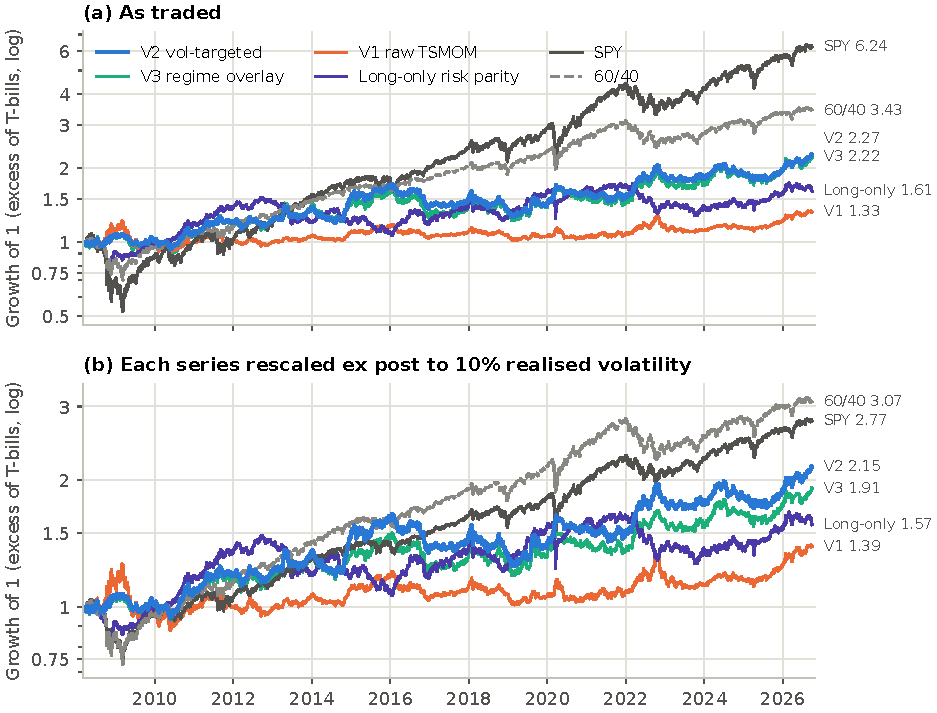
\includegraphics[width=\textwidth]{figures/fig01_cumulative.pdf}
\caption{Growth of one unit invested in each strategy, in excess of T-bills (log scale). Panel (b) rescales each series ex post to 10\% realised volatility to compare return per unit of risk; the rescaling uses full-sample information and is not tradable.}
\label{fig:cumulative}
\end{figure}

The gains are economically meaningful but statistically fragile. Table~\ref{tab:sharpe} reports bootstrap tests of Sharpe ratio differences. V2 improves on V1 by 0.19 with a 95\% confidence interval from $-0.11$ to 0.48 ($p = 0.19$). The step from V2a to V2, which adds time-varying portfolio scaling, is the closest to significance ($p = 0.06$), so the time variation in aggregate exposure, rather than the cross-sectional risk balancing alone, is where the marginal improvement sits. The choice between equal risk per asset class and per instrument makes no difference to the Sharpe ratio (Appendix Table~\ref{tab:trials}). This matches the conclusion of \citet{kim2016} that volatility scaling contributes much of TSMOM's apparent performance, with the qualification that in this sample its contribution cannot be distinguished from noise.

\begin{table}[!htbp]
\centering
\caption{Sharpe ratio difference tests. Paired stationary bootstrap of monthly returns (mean block 6 months, 5,000 replications); two-sided $p$-value. Corr.: correlation of the two monthly return series. Tests for every other configuration are in Table~\ref{tab:trials}.}
\label{tab:sharpe}
\small
\begin{tabular}{lrrrcrr}
\toprule
Comparison & SR$_a$ & SR$_b$ & Difference & 95\% CI & $p$ & Corr. \\
\midrule
V2 vol-targeted vs V1 raw TSMOM & 0.45 & 0.26 & +0.19 & [$-$0.11, 0.48] & 0.19 & 0.82 \\
V2a inverse-vol vs V1 raw TSMOM & 0.36 & 0.26 & +0.11 & [$-$0.15, 0.35] & 0.40 & 0.88 \\
V2 vol-targeted vs V2a inverse-vol & 0.45 & 0.36 & +0.09 & [0.00, 0.18] & 0.06 & 0.98 \\
V2 vol-targeted vs Long-only risk parity & 0.45 & 0.29 & +0.16 & [$-$0.48, 0.81] & 0.63 & 0.09 \\
V3 regime (R1) vs V2 vol-targeted & 0.39 & 0.45 & $-$0.06 & [$-$0.17, 0.05] & 0.32 & 0.96 \\
\bottomrule
\end{tabular}

\end{table}

Figure~\ref{fig:drawdowns} shows the drawdowns. V2's maximum drawdown of 26.8\% ran from January 2016 to February 2019 and was not recovered until April 2022: trend following can be unrewarding for years at a time. V1's drawdown, from March 2009, was not recovered until September 2022. Calendar-year returns show the familiar pattern of trend following: strong in 2008, 2010 and 2022, weak in 2009, 2016 and 2018.

\begin{figure}[!htbp]
\centering
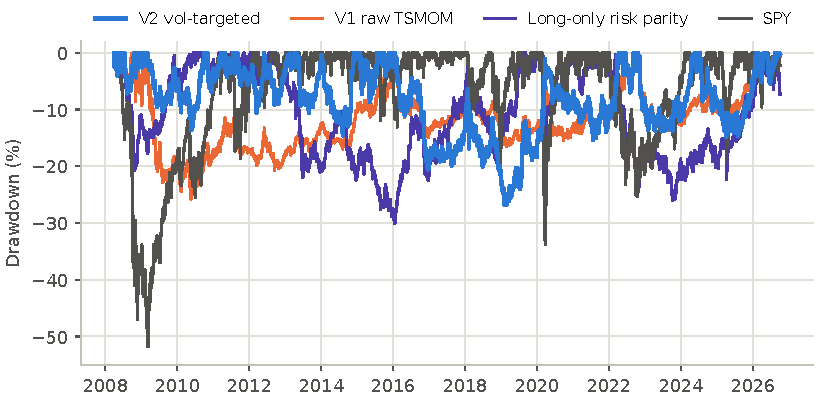
\includegraphics[width=\textwidth]{figures/fig02_drawdowns.pdf}
\caption{Drawdowns of the cumulative excess return, daily.}
\label{fig:drawdowns}
\end{figure}

\subsection{Volatility targeting in practice}

V2 targets 10\% ex-ante volatility but realised 11.27\% (Table~\ref{tab:volval}), a bias statistic of 1.13. The forecasting error is not a code error: the ex-ante volatility of every rebalanced portfolio was verified independently. The overshoot comes from volatility jumps that a backward-looking estimator cannot anticipate, concentrated in September and October 2008, October 2014, February 2018 and March 2020. Figure~\ref{fig:vollev} shows twelve-month rolling realised volatility ranging from about 5\% to 17\%. The same overshoot appears in long-only risk parity (bias statistic 1.10), so it is a property of the risk model rather than of the trend signal.

\begin{table}[!htbp]
\centering
\caption{Accuracy of the volatility forecast. Ex-ante vol is the mean forecast at rebalance; the bias statistic is the standard deviation of monthly returns divided by the ex-ante monthly volatility. Given the kurtosis of V2's standardised returns, the standard error of its bias statistic is about 0.05. $|z|$: absolute standardised monthly return.}
\label{tab:volval}
\tabfit{tables/tab14_vol_validation}
\end{table}

The price of the target is leverage. V2's gross leverage averages 2.15 times net asset value; its 95th percentile is 3.38, it exceeds 3 in 12\% of months, and it peaks at 4.58 in the low-volatility spring of 2013. For futures this is unremarkable; for an ETF implementation it implies margin financing and short borrowing, whose costs are examined in Section~\ref{sec:costs}. Table~\ref{tab:riskshares} shows how the allocation changes the source of risk. Under V1, equities supply 48.5\% of ex-ante portfolio variance; under V2, each asset class supplies between 20.6\% and 32.6\%, with rates the largest because IEF and TLT usually hold same-sign positions.

\begin{table}[!htbp]
\centering
\caption{Average share of ex-ante portfolio variance by asset class (\%). V2 per-instrument gives each instrument an equal risk budget instead of each asset class.}
\label{tab:riskshares}
\small
\begin{tabular}{lrrr}
\toprule
Asset class & V1 & V2 & V2 per-instrument \\
\midrule
Equity & 48.5 & 22.8 & 32.6 \\
Rates & 14.0 & 32.6 & 22.3 \\
Commodity & 22.5 & 24.0 & 17.1 \\
FX & 15.1 & 20.6 & 28.0 \\
\bottomrule
\end{tabular}

\end{table}

\begin{figure}[!htbp]
\centering
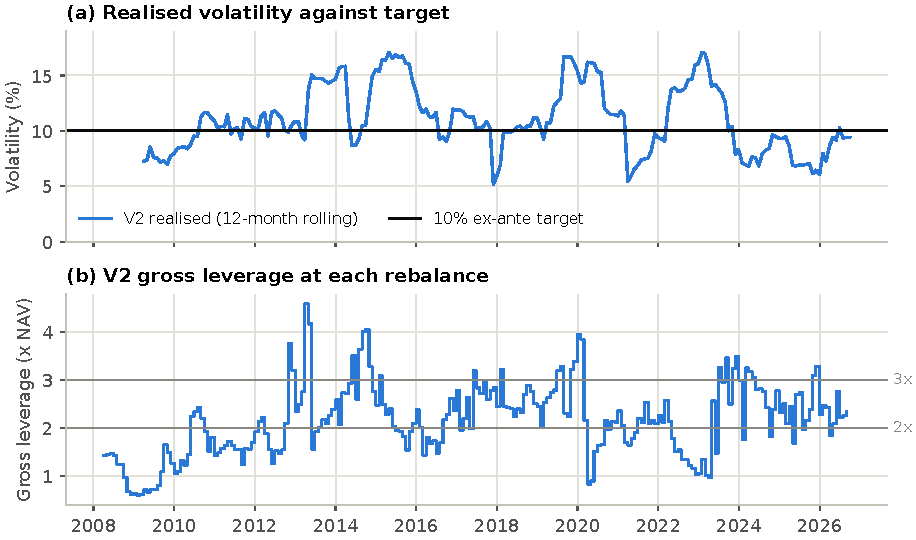
\includegraphics[width=\textwidth]{figures/fig08_vol_leverage.pdf}
\caption{(a) Twelve-month rolling realised volatility of V2 against the 10\% ex-ante target. (b) V2 gross leverage at each monthly rebalance.}
\label{fig:vollev}
\end{figure}

\subsection{Is it trend, static exposure, or the futures factor?}

Table~\ref{tab:spanning} reports spanning regressions. Regressed on SPY, V2 has a slightly negative beta ($-0.10$) and an annualised alpha of 6.21\% ($t = 2.25$). This alpha $t$-statistic exceeds the $t$-statistic of V2's raw mean because the negative equity beta is credited for SPY's strong return; it should not be read as significant stand-alone alpha. Against long-only risk parity, the more demanding benchmark, the alpha falls to 4.78\% ($t = 1.76$). V2's correlation with LO-RP is only 0.09, so the trend signal is not a disguised static risk-parity position, but the comparison is noisy and the Sharpe difference between them is insignificant (Table~\ref{tab:sharpe}).

\begin{table}[!htbp]
\centering
\caption{Spanning regressions of monthly excess returns, $y_t = \alpha + \beta f_t + e_t$. Alpha annualised; Newey-West $t$-statistics. Benchmark regressions use 222 months; the AQR regressions use the 218 months to May 2026, aligned by calendar month. Correlations of V2's asset-class sleeves with the corresponding AQR asset-class factors: rates 0.83, currencies 0.69, commodities 0.65, equities 0.63.}
\label{tab:spanning}
\small
\begin{tabular}{llrrrr}
\toprule
Strategy & Benchmark & $\alpha$ (\%/yr) & $t(\alpha)$ & $\beta$ & $R^2$ \\
\midrule
V2 & SPY & 6.21 & 2.25 & $-$0.10 & 0.02 \\
V2 & 60/40 & 5.95 & 2.14 & $-$0.12 & 0.01 \\
V2 & LO-RP & 4.78 & 1.76 & 0.09 & 0.01 \\
V1 & AQR TSMOM & $-$0.38 & $-$0.31 & 0.40 & 0.58 \\
V2 & AQR TSMOM & 1.37 & 0.88 & 0.66 & 0.60 \\
\bottomrule
\end{tabular}

\end{table}

The AQR factor provides external validation. V2 has a beta of 0.66 on the AQR TSMOM factor, an $R^2$ of 0.60 (a correlation of 0.77) and an insignificant alpha of 1.37\% a year, and each asset-class sleeve is positively correlated with the corresponding AQR sleeve. A ten-ETF portfolio therefore reproduces most of the variation of a 58-instrument futures strategy: the implementation captures the same economic phenomenon, and any shortfall in its returns reflects narrower breadth rather than a different strategy.

\subsection{Crisis performance}

Crisis windows are defined by a rule rather than chosen by eye: every peak-to-trough decline of more than 15\% in SPY's total-return index, measured from its running maximum within the sample. The rule yields six windows (Table~\ref{tab:crisis}). The 2010 decline of 15.7\% is not a separate window because SPY had not yet regained its 2008 peak.

\begin{table}[!htbp]
\centering
\caption{Crisis windows: every SPY total-return drawdown deeper than 15\% from its running high, April 2008 to September 2026. SPY drawdown defines the window; the remaining columns are cumulative excess returns over T-bills from the day after the peak to the trough (\%). Lower rows: mean monthly or quarterly excess return (\%) in SPY's worst decile of months and quarters.}
\label{tab:crisis}
\small
\begin{tabular}{llrrrrrrrrr}
\toprule
& & SPY & \multicolumn{8}{c}{Excess return over the window (\%)} \\
\cmidrule(lr){4-11}
Peak & Trough & drawdown & SPY & V1 & V2 & V3 & LO-RP & 60/40 & 60/40 + V2 & SPY + V2 \\
\midrule
2008-05-19 & 2009-03-09 & $-$51.5 & $-$51.8 & 21.3 & 9.2 & 10.1 & $-$16.9 & $-$32.3 & $-$25.3 & $-$42.7 \\
2011-04-29 & 2011-10-03 & $-$18.6 & $-$18.6 & $-$6.5 & $-$1.2 & $-$2.3 & 3.5 & $-$6.7 & $-$5.6 & $-$15.3 \\
2018-09-20 & 2018-12-24 & $-$19.3 & $-$19.8 & $-$2.5 & $-$7.4 & $-$7.1 & $-$4.7 & $-$11.1 & $-$10.3 & $-$17.3 \\
2020-02-19 & 2020-03-23 & $-$33.7 & $-$33.8 & 6.6 & 12.6 & 9.0 & $-$17.9 & $-$18.9 & $-$12.9 & $-$25.3 \\
2022-01-03 & 2022-10-12 & $-$24.5 & $-$25.3 & 16.6 & 30.6 & 29.0 & $-$20.8 & $-$21.6 & $-$12.6 & $-$15.8 \\
2025-02-19 & 2025-04-08 & $-$18.8 & $-$19.2 & $-$3.1 & $-$4.1 & $-$5.6 & $-$8.2 & $-$11.1 & $-$9.7 & $-$16.3 \\
\midrule
\multicolumn{3}{l}{SPY worst-decile months, mean ($n=23$)} & $-$8.1 & 1.4 & 1.8 & 1.5 & $-$2.6 & $-$4.7 & $-$3.4 & $-$6.1 \\
\multicolumn{3}{l}{SPY worst-decile quarters, mean ($n=8$)} & $-$14.7 & 1.2 & 2.8 & 2.0 & $-$3.2 & $-$7.2 & $-$5.2 & $-$11.3 \\
\bottomrule
\end{tabular}

\end{table}

V2 was positive in the three largest drawdowns, gaining 9.2\% from May 2008 to March 2009 (SPY $-51.8\%$), 12.6\% in the February to March 2020 crash (SPY $-33.8\%$) and 30.6\% over the 2022 inflation shock (SPY $-25.3\%$). It lost in the three shorter, sharper episodes of 2011, late 2018 and early 2025, when twelve-month signals were still positioned for the preceding rally. Figure~\ref{fig:crisis} shows the daily paths. In SPY's worst decile of months, V2 averaged $+1.8\%$ against $-8.1\%$ for SPY; long-only risk parity averaged $-2.6\%$. Trend following tends to give back part of these gains in the recovery: V2 lost 5.7\% from March to August 2020 and 8.7\% between the October 2022 trough and SPY's new high in December 2023.

\begin{figure}[!htbp]
\centering
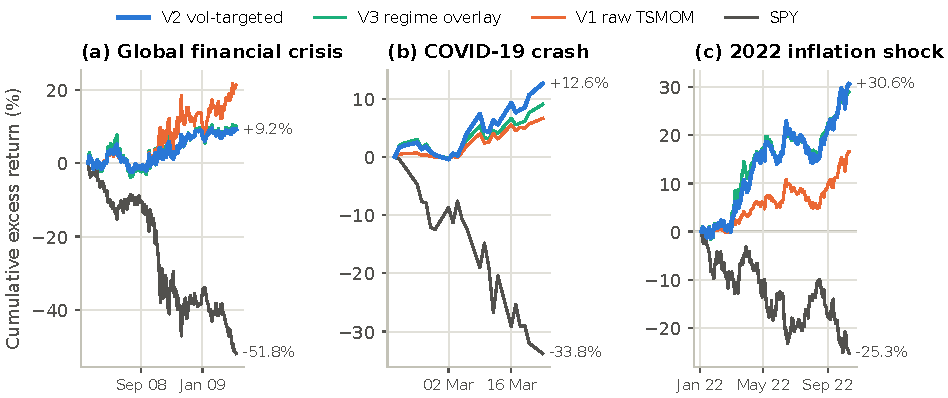
\includegraphics[width=\textwidth]{figures/fig03_crisis_zooms.pdf}
\caption{Cumulative excess return from the SPY peak to the trough in the three largest drawdowns.}
\label{fig:crisis}
\end{figure}

The 2020 result contradicts a common expectation, which was also my prior: that trend followers lose in fast crashes because their twelve-month signals are still long equities. An attribution of V2's return from 20 February to 23 March 2020 shows why it did not. The equity sleeve was mixed (long SPY, short EEM, with EFA switching from long to short at the end of February) and lost only 1.2\% in total, while the rest of the book was already positioned defensively: long Treasuries ($+6.6\%$), short the commodity basket ($+4.5\%$ from commodities) and long the dollar against the Australian dollar ($+2.5\%$ from currencies). Equal risk per asset class limited the damage from the one sleeve that was wrong. The same episode exposes static risk parity: on 18 March 2020 equities, Treasuries, gold and commodities fell together, and LO-RP lost 6.8\% in a day.

Figure~\ref{fig:smile} plots quarterly V2 returns against quarterly SPY returns, the ``smile'' that \citet{fung2001} associate with trend followers, whose payoff resembles a long straddle. The fitted quadratic coefficient is positive (0.67) but not significant ($t = 1.20$, 74 quarters), so the convexity is visible but statistically weak in this sample.

\begin{figure}[!htbp]
\centering
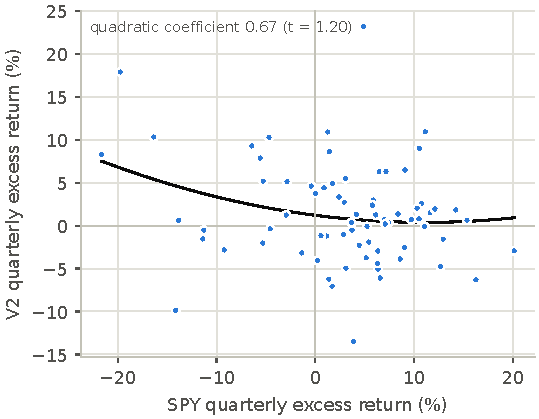
\includegraphics[width=0.62\textwidth]{figures/fig07_smile.pdf}
\caption{Quarterly V2 excess returns against quarterly SPY excess returns (74 quarters) with the fitted quadratic $r_q = a + b\,\mathrm{SPY}_q + c\,\mathrm{SPY}_q^2$; Newey-West $t$-statistic.}
\label{fig:smile}
\end{figure}

\subsection{Trend following as a portfolio diversifier}
\label{sec:blend}

V2's Sharpe ratio of 0.45 is below those of SPY (0.72) and the 60/40 portfolio (0.74), so the case for holding it rests on its role as a diversifier. This subsection tests that role directly. It was added after the results above had been seen, and its specification was committed before it was computed. It uses V2 exactly as reported, so it does not add a trend configuration to the trial count of Section~\ref{sec:dsr}.

\textbf{Design.} The primary portfolio holds 80\% in the 60/40 benchmark and 20\% in V2; a secondary portfolio holds 80\% in SPY and 20\% in V2. Allocations of 10\% to 20\% to managed futures are common, and 20\% was fixed in advance; no other weight was computed. The sleeves are reset to their target weights at each month-end and drift within the month, so daily drawdowns are measured as in Table~\ref{tab:perf}. V2 is net of costs while the benchmarks are gross; the blend's own rebalancing (0.13 of net asset value a year) is not charged. The specification names drawdowns and crisis losses as the headline, because that is the purpose of a diversifier.

\begin{table}[!htbp]
\centering
\caption{Trend following held beside conventional portfolios, April 2008 to September 2026 (222 months). Blends hold 80\% in the benchmark and 20\% in V2, rebalanced monthly with daily drift. Mean and volatility are annualised excess returns over T-bills (\%); the maximum drawdown (MDD, \%) and its recovery date are from daily data. Corr.\ is the monthly correlation of V2 with the benchmark. $\Delta$SR is the Sharpe ratio of the blend minus that of its benchmark, with a two-sided paired stationary bootstrap $p$-value. Turn.\ is the net asset value moved between sleeves per year. V2 is net of 10 basis points; the benchmarks are gross of costs.}
\label{tab:blend}
\footnotesize
\setlength{\tabcolsep}{3.3pt}
\begin{tabular}{lrrrrrccccrrrrr}
\toprule
& & & & & \multicolumn{4}{c}{Maximum drawdown} & & & & \multicolumn{2}{c}{vs benchmark} & \\
\cmidrule(lr){6-9} \cmidrule(lr){13-14}
 & Mean & Vol & Sharpe & (SE) & MDD & Peak & Trough & Recovery & Calmar & Skew$_m$ & Corr. & $\Delta$SR & $p$ & Turn. \\
\midrule
\multicolumn{15}{l}{\textit{Primary: 60/40 investor}} \\
60/40 & 7.15 & 9.65 & 0.74 & (0.24) & $-$32.3 & 2008-05-19 & 2009-03-09 & 2010-10-05 & 0.22 & $-$0.62 & $-$0.11 &  &  &  \\
80\% 60/40 + 20\% V2 & 6.74 & 7.81 & 0.86 & (0.24) & $-$25.3 & 2008-05-19 & 2009-03-09 & 2010-09-20 & 0.27 & $-$0.47 & -- & +0.12 & 0.08 & 0.13 \\
\addlinespace
\multicolumn{15}{l}{\textit{Secondary: equity-only investor}} \\
SPY & 11.18 & 15.61 & 0.72 & (0.23) & $-$51.8 & 2008-05-19 & 2009-03-09 & 2011-04-27 & 0.22 & $-$0.58 & $-$0.14 &  &  &  \\
80\% SPY + 20\% V2 & 9.95 & 12.37 & 0.80 & (0.24) & $-$42.7 & 2008-05-19 & 2009-03-09 & 2011-01-27 & 0.23 & $-$0.50 & -- & +0.09 & 0.04 & 0.17 \\
\bottomrule
\end{tabular}

\end{table}

\textbf{Results.} V2's monthly correlation with the 60/40 portfolio is $-0.11$. Adding it at 20\% lowers the 60/40 portfolio's volatility from 9.65\% to 7.81\% and its mean less, from 7.15\% to 6.74\%, so the Sharpe ratio rises from 0.74 to 0.86. The maximum drawdown falls from 32.3\% to 25.3\%. For the equity-only investor it falls from 51.8\% to 42.7\%, and the Sharpe ratio rises from 0.72 to 0.80. In each of the six crisis windows, for both investors, the blend lost less than its benchmark (Table~\ref{tab:blendcrisis}). The largest reductions came when V2 itself made money: the 60/40 investor's loss fell from 18.9\% to 12.9\% in 2020 and from 21.6\% to 12.6\% in 2022. The reductions in 2011, 2018 and 2025 were small (0.8 to 1.4 percentage points) and come mainly from holding 20\% less of the benchmark. Figure~\ref{fig:blend} shows the full paths.

\begin{table}[!htbp]
\centering
\caption{Crisis windows (as in Table~\ref{tab:crisis}): cumulative excess return over T-bills from the day after the SPY peak to the trough (\%), for each benchmark and its 80/20 blend with V2. Change is the blend minus the benchmark in percentage points. Lower rows: mean excess return in SPY's worst decile of months and quarters.}
\label{tab:blendcrisis}
\small
\begin{tabular}{llrrrrrr}
\toprule
& & \multicolumn{3}{c}{60/40 investor} & \multicolumn{3}{c}{Equity-only investor} \\
\cmidrule(lr){3-5} \cmidrule(lr){6-8}
Peak & Trough & 60/40 & Blend & Change & SPY & Blend & Change \\
\midrule
2008-05-19 & 2009-03-09 & $-$32.3 & $-$25.3 & +7.1 & $-$51.8 & $-$42.7 & +9.1 \\
2011-04-29 & 2011-10-03 & $-$6.7 & $-$5.6 & +1.1 & $-$18.6 & $-$15.3 & +3.3 \\
2018-09-20 & 2018-12-24 & $-$11.1 & $-$10.3 & +0.8 & $-$19.8 & $-$17.3 & +2.5 \\
2020-02-19 & 2020-03-23 & $-$18.9 & $-$12.9 & +6.0 & $-$33.8 & $-$25.3 & +8.5 \\
2022-01-03 & 2022-10-12 & $-$21.6 & $-$12.6 & +9.0 & $-$25.3 & $-$15.8 & +9.5 \\
2025-02-19 & 2025-04-08 & $-$11.1 & $-$9.7 & +1.4 & $-$19.2 & $-$16.3 & +2.9 \\
\midrule
\multicolumn{2}{l}{SPY worst-decile months, mean ($n=23$)} & $-$4.7 & $-$3.4 & +1.3 & $-$8.1 & $-$6.1 & +2.0 \\
\multicolumn{2}{l}{SPY worst-decile quarters, mean ($n=8$)} & $-$7.2 & $-$5.2 & +1.9 & $-$14.7 & $-$11.3 & +3.4 \\
\bottomrule
\end{tabular}

\end{table}

\begin{figure}[!htbp]
\centering
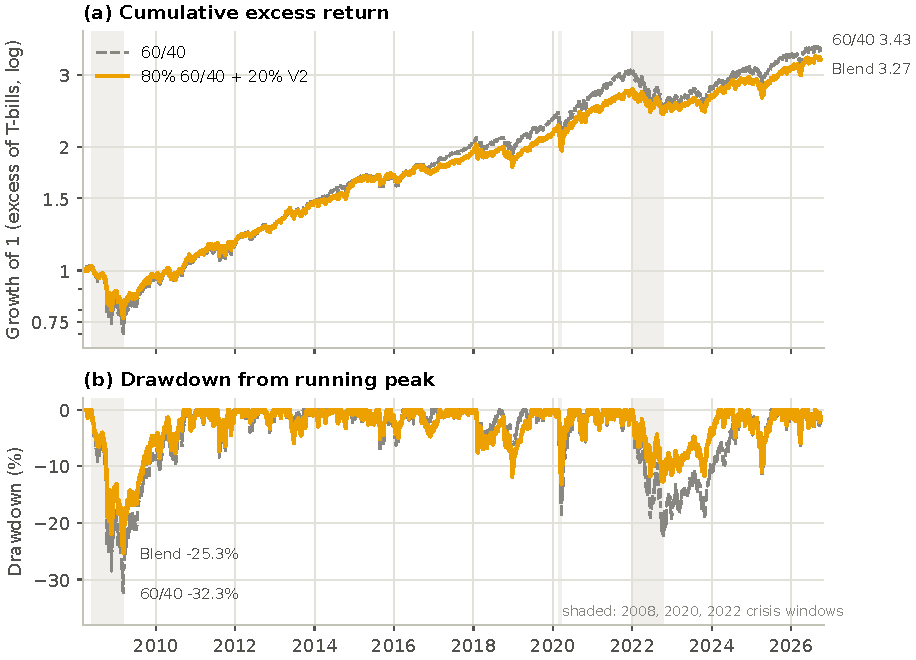
\includegraphics[width=\textwidth]{figures/fig10_blend.pdf}
\caption{The 60/40 portfolio and the blend of 80\% 60/40 and 20\% V2, daily: (a) growth of one unit in excess of T-bills (log scale); (b) drawdown from the running peak. Shaded: the 2008, 2020 and 2022 crisis windows.}
\label{fig:blend}
\end{figure}

\textbf{Statistical significance.} The improvement in the Sharpe ratio is not significant for the primary blend: the difference is 0.12 with a bootstrap $p$-value of 0.08. For the equity-only blend the difference of 0.09 has $p = 0.04$, but two blends were tested, and a Bonferroni adjustment for the pair would put it at 0.08. The evidence therefore supports a narrower claim than ``trend following improves a portfolio'': over this sample, a fixed 20\% allocation to V2 reduced drawdowns and crisis losses in every episode, at the cost of a lower mean return, and the rise in the risk-adjusted return is consistent with that benefit but not statistically established.

\subsection{The regime overlay}
\label{sec:regime_results}

Table~\ref{tab:regime} evaluates the overlay. V3 lowers the Sharpe ratio from 0.45 to 0.39 ($p = 0.32$). Regressed on V2, it has a beta of 1.12 and a negative, insignificant alpha: the overlay mainly raises average exposure (its mean multiplier is 1.19) without improving its timing.

\textbf{Holding exposure constant.} Because V3's multiplier averages 1.19, the comparison with V2 mixes a change in the level of exposure with a change in its timing. Two checks, added after the results above had been seen and specified before they were computed, separate the two. The first divides the multiplier by its own walk-forward average, $m_t = (0.5 + p_t)/(0.5 + \bar p_t)$, where $\bar p_t$ is the mean of the target-state probabilities from the first refit up to and including month $t$, so it uses no future data; dividing by the full-sample mean instead would be a lookahead error. Its Sharpe ratio is 0.40, 0.05 below V2's ($p = 0.33$), its alpha on V2 is negative, and the normalised multiplier does not forecast V2's returns (Table~\ref{tab:regime_pred}). The second scales V2 by the constant 1.19, which uses full-sample information and is not tradable; it has V2's Sharpe ratio by construction, and V3 falls 0.06 short of it ($p = 0.32$). Under the rule fixed in advance, the conclusion that the overlay adds no timing value is confirmed. The normalised multiplier averages 0.93 rather than one, because its expanding mean starts close to one during the degenerate fits of 2008 to 2010 (described below), so its smaller maximum drawdown (21.5\%) reflects lower average exposure rather than better timing.

\begin{table}[!htbp]
\centering
\caption{Regime-conditioned exposure. $\Delta$SR and $p$: Sharpe difference from V2 and bootstrap $p$-value. $\alpha$ on V2: annualised alpha (\%) from regressing the overlay on V2, Newey-West $t$. V3 normalised divides the V3 multiplier by its walk-forward mean. $^\ddagger$Scales V2 by V3's realised mean multiplier, which uses full-sample information: a diagnostic, not a tradable strategy, with V2's Sharpe ratio by construction, so no test is reported. $^\dagger$Lookahead illustrations use a single full-sample fit and therefore future data; they are not results. Other overlay variants are in Table~\ref{tab:regimeextra}.}
\label{tab:regime}
\small
\tabfit{tables/tab08_regime}
\end{table}

Two diagnostics explain the failure. First, the states are not what the labels suggest. In every non-degenerate refit, the higher-mean ``trending'' state of the trend payoff is also its lower-variance state: the model separates calm periods with a positive payoff from volatile periods with a slightly negative one, so it behaves largely as a volatility filter on the trend payoff. Second, the label does not forecast returns. Table~\ref{tab:regime_pred} regresses V2's next-month return on the probability: the slope is negative ($t = -0.74$), and in months the model calls ``trending'' V2's Sharpe ratio is 0.33, against 0.80 in the others. Figure~\ref{fig:regimes} shows the probabilities over time.

\begin{table}[!htbp]
\centering
\caption{Does the regime probability forecast trend returns? V2's return in month $t+1$ regressed on the target-state probability $p_t$ (slope in \% per month per unit of probability; Newey-West $t$), and V2's annualised Sharpe ratio in months with $p_t$ above and below 0.5. $^\ddagger$Regressor is the normalised multiplier $m_t$ (slope per unit of multiplier), split at $m_t > 1$. $^\dagger$Uses future data.}
\label{tab:regime_pred}
\small
\begin{tabular}{lrrrrrr}
\toprule
& & & \multicolumn{2}{c}{$p_t > 0.5$} & \multicolumn{2}{c}{$p_t \le 0.5$} \\
\cmidrule(lr){4-5}\cmidrule(lr){6-7}
Model & Slope & $t$ & Sharpe & Months & Sharpe & Months \\
\midrule
R1 primary & $-$0.72 & $-$0.74 & 0.33 & 176 & 0.80 & 46 \\
R1 normalised$^\ddagger$ & $-$0.93 & $-$0.71 & 0.31 & 101 & 0.55 & 121 \\
R1 smoothed$^\dagger$ & 0.91 & 1.30 & 0.83 & 117 & 0.13 & 105 \\
\bottomrule
\end{tabular}

\end{table}

\begin{figure}[!htbp]
\centering
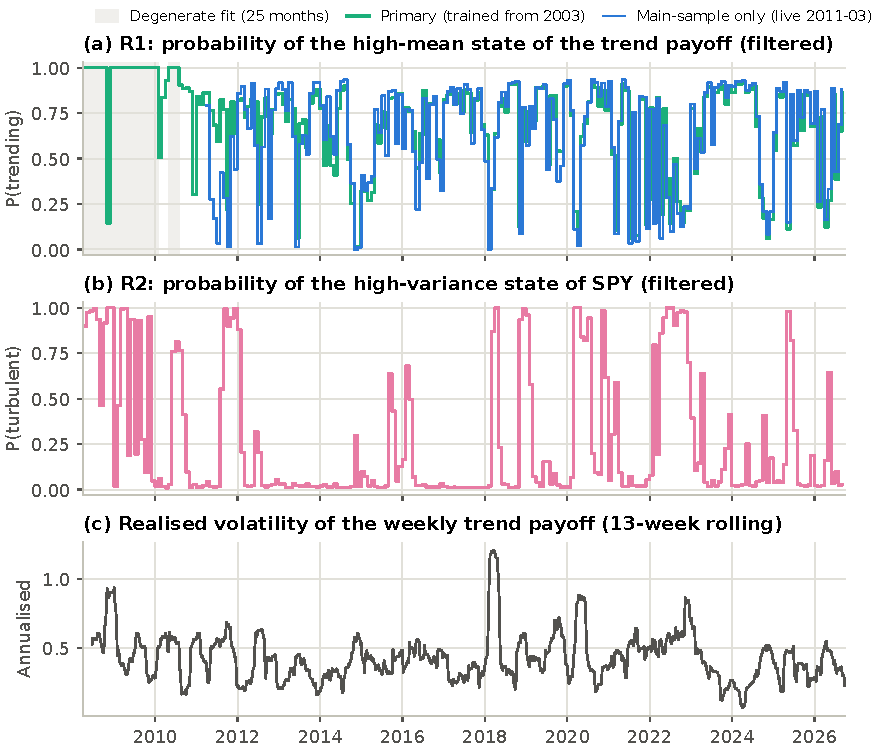
\includegraphics[width=\textwidth]{figures/fig04_regimes.pdf}
\caption{(a) Walk-forward filtered probability of the trending state, set at each month-end and held over the following month, with the holding months of the 25 degenerate fits shaded. (b) Realised volatility of the weekly trend payoff.}
\label{fig:regimes}
\end{figure}

\textbf{Degenerate fits.} In 25 of the first 27 monthly refits (March 2008 to June 2010), the maximum-likelihood estimate devotes one state to a handful of isolated extreme weeks from the burn-in period: that state has a mean payoff of about $-0.27$ per week, against a full-sample weekly standard deviation of 0.07, and a probability of persisting of zero. This is a known weakness of maximum likelihood for mixtures of normal distributions, whose likelihood rewards fitting individual extreme observations \citep{kiefer1978,hamilton1991}. With the outliers absorbed, the remaining state was labelled ``trending'' with probability close to one, so V3 held 1.5 times V2's exposure through 2008 to 2010; no degenerate fit occurs after June 2010. The pre-registered result is reported unchanged. A diagnostic variant defined after the problem was found, which sets the multiplier to one at degenerate refits, still trails V2 (Sharpe 0.42; Appendix~\ref{app:trials}).

\textbf{The cost of lookahead.} The same overlay computed from full-sample smoothed probabilities would have reported a Sharpe ratio of 0.57, a gain of 0.12 over V2, a maximum drawdown of 18.7\% instead of 26.8\%, and a positive predictive slope. Using full-sample parameters with filtered probabilities produces no such gain (0.43). Almost all of the spurious improvement therefore comes from smoothing, which conditions each week's state on future observations, rather than from estimating the parameters on the full sample. An overlay that looks valuable in-sample and worthless out-of-sample is the typical signature of this error, and the gap of 0.18 between the smoothed and walk-forward versions measures how large it can be.

\section{Robustness and Validation}
\label{sec:robust}

\subsection{Signal horizon}

Figure~\ref{fig:horizons} reports V2 at each lookback. The ordering matches the literature: the one-month signal loses money (Sharpe $-0.20$) with a turnover of 28.9 times a year, and performance improves with the horizon to 0.45 at twelve months. The blend of all four horizons earns 0.43. The 95\% confidence intervals overlap heavily, so the evidence ranks the horizons only loosely; the twelve-month primary was fixed in advance and was not selected for being the best.

\begin{figure}[!htbp]
\centering
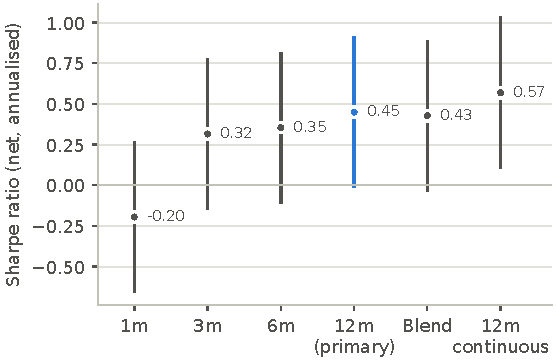
\includegraphics[width=0.62\textwidth]{figures/fig06_horizons.pdf}
\caption{V2 Sharpe ratio by signal, net of costs, with 95\% intervals from Lo (2002) standard errors. The intervals are not independent: all variants share the same instruments and sample.}
\label{fig:horizons}
\end{figure}

\subsection{Robustness grid}

Table~\ref{tab:robust} varies one element of V2 at a time. Every variant is reported and none was selected; the rows not shown here are in Appendix Table~\ref{tab:trials}. A one-day execution lag leaves the Sharpe ratio unchanged (0.45), so the results do not depend on trading at the signal close. Capping gross leverage at 2 times reduces the Sharpe ratio to 0.41 and volatility to 9.4\%. A faster volatility estimator (centre of mass 20 days) lowers the Sharpe ratio to 0.40 ($p = 0.08$) and widens rather than narrows the volatility overshoot (bias statistic 1.19), so the overshoot is not a matter of a slow estimator. A continuous signal, $\mathrm{clip}(t_{i,t}/2, -1, 1)$ where $t_{i,t}$ is the $t$-statistic of the mean daily excess return over the past twelve months \citep{baltas2013}, has the highest point estimate in the grid (0.57), but the difference from V2 is insignificant ($p = 0.22$). It was specified during the robustness analysis, before its result was computed, and it was not adopted.

\begin{table}[!htbp]
\centering
\caption{Robustness grid: V2 with one element changed. $\Delta$SR and $p$: Sharpe difference from V2 and bootstrap $p$-value. Corr.: correlation with V2. Vol and MDD in \%. Vol bias: bias statistic of the variant's own ex-ante volatility forecast. All net of 10 bps.}
\label{tab:robust}
\small
\begin{tabular}{lrrrrrrrr}
\toprule
Variant & Sharpe & $\Delta$SR & $p$ & Corr. & Vol & MDD & Turn. & Vol bias \\
\midrule
Primary (V2) & 0.45 & -- & -- & 1.00 & 11.3 & $-$26.8 & 9.8 & 1.13 \\
\addlinespace
\multicolumn{9}{l}{\textit{Implementation and estimation}} \\
Execution lag 1 day & 0.45 & +0.00 & 0.92 & 0.99 & 11.1 & $-$30.5 & 9.8 & 1.11 \\
EWMA centre of mass 20 days & 0.40 & $-$0.05 & 0.08 & 0.99 & 11.9 & $-$27.3 & 11.7 & 1.19 \\
EWMA centre of mass 120 days & 0.46 & +0.01 & 0.48 & 1.00 & 11.0 & $-$27.9 & 9.0 & 1.10 \\
Gross leverage cap 2$\times$ & 0.41 & $-$0.04 & 0.29 & 0.98 & 9.4 & $-$22.4 & 6.6 & 1.13 \\
\addlinespace
\multicolumn{9}{l}{\textit{Signal}} \\
Continuous $t$-statistic signal & 0.57 & +0.12 & 0.22 & 0.94 & 11.6 & $-$24.3 & 8.4 & 1.16 \\
\addlinespace
\multicolumn{9}{l}{\textit{Leave one asset class out}} \\
Excluding equity & 0.29 & $-$0.16 & 0.09 & 0.93 & 11.5 & $-$35.0 & 9.9 & 1.15 \\
Excluding rates & 0.41 & $-$0.04 & 0.77 & 0.85 & 10.5 & $-$26.6 & 9.6 & 1.05 \\
Excluding commodities & 0.34 & $-$0.11 & 0.25 & 0.92 & 10.9 & $-$21.6 & 9.3 & 1.09 \\
Excluding FX & 0.50 & +0.05 & 0.52 & 0.94 & 10.6 & $-$28.8 & 7.3 & 1.06 \\
\bottomrule
\end{tabular}

\end{table}

Leaving out one asset class at a time shows where the returns come from. Removing equities lowers the Sharpe ratio most (to 0.29, $p = 0.09$), followed by commodities (0.34). Removing currencies raises it to 0.50, consistent with the weak trends of the currency sleeve, although the difference is again insignificant. No single asset class drives the result, but equity and commodity trends contributed most.

\subsection{Subperiods}

Table~\ref{tab:halves} splits the sample into two halves of 111 months. V2's Sharpe ratio is 0.38 in the first half and 0.52 in the second, positive in both and well within one standard error (0.33) of each other. The regime overlay is unstable across halves: V3 is weaker than V2 in the first half, when the degenerate fits occurred (0.27 against 0.38), and slightly stronger in the second (0.53 against 0.52). SPY's Sharpe ratio exceeds V2's in both halves.

\begin{table}[!htbp]
\centering
\caption{Subperiod halves of 111 months each. Annualised mean excess return (\%) and Sharpe ratio with Lo (2002) standard error.}
\label{tab:halves}
\small
\begin{tabular}{lrrrrrr}
\toprule
& \multicolumn{3}{c}{2008-04 to 2017-06} & \multicolumn{3}{c}{2017-07 to 2026-09} \\
\cmidrule(lr){2-4}\cmidrule(lr){5-7}
 & Mean & Sharpe & (SE) & Mean & Sharpe & (SE) \\
\midrule
V1 raw TSMOM & 1.00 & 0.13 & (0.33) & 2.58 & 0.41 & (0.33) \\
V2 vol-targeted & 4.36 & 0.38 & (0.33) & 5.77 & 0.52 & (0.33) \\
V3 regime (R1) & 3.77 & 0.27 & (0.33) & 6.58 & 0.53 & (0.33) \\
Long-only risk parity & 3.44 & 0.30 & (0.33) & 2.95 & 0.28 & (0.33) \\
SPY & 9.65 & 0.63 & (0.33) & 12.70 & 0.80 & (0.33) \\
60/40 & 7.45 & 0.83 & (0.33) & 6.86 & 0.66 & (0.33) \\
\bottomrule
\end{tabular}

\end{table}

\subsection{Costs, borrowing and financing}
\label{sec:costs}

Table~\ref{tab:costs} and Figure~\ref{fig:costs} show the effect of trading costs. V2 trades 9.8 times its net asset value a year, so each basis point of one-way cost costs about 0.1\% a year. Its Sharpe ratio is 0.54 before costs, 0.45 at the assumed 10 basis points and 0.10 at 50 basis points; its break-even cost is 62 basis points per unit traded, well above the cost of trading these funds. The regime overlay raises turnover to 14.2 and lowers the break-even to 47 basis points. Long-only risk parity, which trades little, overtakes V2 at costs above about 30 basis points.

\begin{table}[!htbp]
\centering
\caption{Cost sensitivity. Annual turnover (multiples of NAV), Sharpe ratio at each one-way cost per unit of notional traded, and the linear break-even cost (annual gross mean excess return divided by annual turnover).}
\label{tab:costs}
\small
\begin{tabular}{lrrrrrrrr}
\toprule
& & \multicolumn{6}{c}{Sharpe ratio at one-way cost (bps)} & \\
\cmidrule(lr){3-8}
 & Turnover & 0 & 2 & 5 & 10 & 20 & 50 & Break-even (bps) \\
\midrule
V1 raw TSMOM & 3.1 & 0.30 & 0.29 & 0.28 & 0.26 & 0.21 & 0.08 & 68 \\
V2a inverse-vol & 3.3 & 0.43 & 0.42 & 0.40 & 0.36 & 0.29 & 0.09 & 64 \\
V2 vol-targeted & 9.8 & 0.54 & 0.52 & 0.49 & 0.45 & 0.36 & 0.10 & 62 \\
V3 regime (R1) & 14.2 & 0.50 & 0.48 & 0.45 & 0.39 & 0.28 & $-$0.04 & 47 \\
V3-R2 regime (SPY) & 8.5 & 0.41 & 0.40 & 0.37 & 0.32 & 0.23 & $-$0.03 & 47 \\
Long-only risk parity & 1.9 & 0.31 & 0.31 & 0.30 & 0.29 & 0.27 & 0.22 & 177 \\
\bottomrule
\end{tabular}

\end{table}

\begin{figure}[!htbp]
\centering
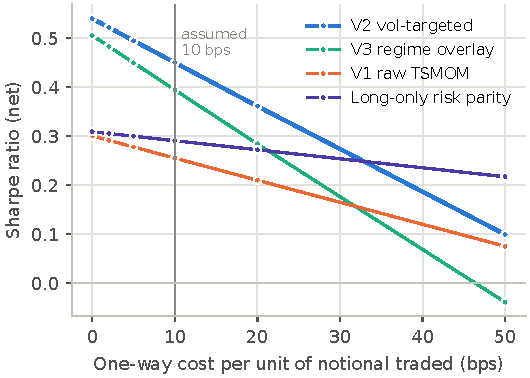
\includegraphics[width=0.62\textwidth]{figures/fig09_costs.pdf}
\caption{Sharpe ratio against one-way trading cost. The vertical line marks the 10 bps assumption.}
\label{fig:costs}
\end{figure}

Financing assumptions matter more than trading costs for an ETF implementation. V2 holds short positions averaging 0.98 times net asset value, and a borrow fee of 100 basis points a year lowers its Sharpe ratio from 0.45 to 0.36. A financing spread of 100 basis points over the bill rate on borrowed cash, which averages 0.33 times net asset value, lowers it to 0.42, and with both at 100 basis points the Sharpe ratio is 0.33.

\subsection{Multiple testing}
\label{sec:dsr}

Twenty-five distinct TSMOM configurations were examined in the original study: V1 at four horizons, V2a, four versions of the regime overlay and the sixteen rows of the robustness grid (the lookahead illustrations are excluded). The cross-sectional standard deviation of their Sharpe ratios is 0.17. Against this background, the probability that V2's true Sharpe ratio exceeds zero, adjusted for non-normality but not for selection, is 0.975. The deflated Sharpe ratio, which asks instead whether V2 beats the best Sharpe ratio expected from $N$ independent trials with no true skill, is 0.68 for $N = 25$ (Table~\ref{tab:dsr}). Because the configurations are highly correlated, the effective number of independent trials is well below 25; but even with $N = 2$ the deflated Sharpe ratio is 0.94, below the conventional 0.95 threshold. The exposure-normalised overlay of Section~\ref{sec:regime_results}, added later, is a twenty-sixth configuration; with it in the trial set the deflated Sharpe ratio is unchanged at 0.68. Every configuration in the trial count is listed, with its Sharpe ratio and its test against V2, in Appendix Table~\ref{tab:trials}. The primary result is therefore suggestive rather than statistically established, a conclusion consistent with the cautions of \citet{harvey2016} on backtested performance. The portfolio blends of Section~\ref{sec:blend} do not change this count: they hold V2 unchanged at a weight fixed in advance, so they test how the existing strategy behaves inside a portfolio rather than adding a new candidate trend strategy from which the best could be selected.

\begin{table}[!htbp]
\centering
\caption{Deflated Sharpe ratio of V2 \citep{bailey2014}. SR$_0$ is the expected maximum annual Sharpe ratio of $N$ independent zero-skill trials, given the observed cross-trial dispersion (0.17); DSR is the probability that V2's true Sharpe ratio exceeds SR$_0$, adjusted for the skewness and kurtosis of its monthly returns. Rows up to $N = 25$ use the dispersion of the original 25 configurations; the $N = 26$ row adds the exposure-normalised overlay to the trial set.}
\label{tab:dsr}
\small
\begin{tabular}{lrr}
\toprule
Number of trials $N$ & SR$_0$ (annual) & DSR \\
\midrule
2 & 0.09 & 0.94 \\
5 & 0.21 & 0.86 \\
10 & 0.27 & 0.78 \\
20 & 0.33 & 0.70 \\
25 (original study) & 0.34 & 0.68 \\
26 (including the normalised overlay) & 0.34 & 0.68 \\
\bottomrule
\end{tabular}

\end{table}

\section{Limitations}
\label{sec:limitations}

\textbf{ETFs are not futures.} A futures implementation would hold margin rather than full notional, finance leverage at close to the bill rate and short without a borrow fee. Here, V2's average gross leverage of 2.15 and short exposure of about one times net asset value require a margin account and a borrow facility, and the fee sensitivities show these costs can remove a quarter of the Sharpe ratio. Margin calls, recall risk on short positions and retail leverage limits are not modelled.

\textbf{Breadth.} Ten instruments, with an effective number of independent bets well below ten, are far fewer than the 58 in MOP. Equities and Treasuries are each close to a single bet, and the three currency funds are correlated. Low breadth makes returns more concentrated and the statistics noisier; the shortfall against the AQR factor is at least partly a breadth effect.

\textbf{One sample, one bond cycle.} The 18.5-year sample contains one long decline in interest rates followed by one sharp rise, and Treasury trends helped in both. A different rate path could produce materially different results. With 222 months the Sharpe ratio standard error is about 0.23, so even a true Sharpe ratio of 0.5 would be hard to distinguish from zero.

\textbf{Volatility forecast.} Realised volatility exceeded the target by 13\%, concentrated in volatility jumps, so a portfolio sized to a risk limit would have breached it in the episodes that matter most. The 60-day volatility and trailing one-year correlations cannot anticipate a sudden change in correlations such as March 2020.

\textbf{Regime model.} The Markov-switching model has limited power with weekly data over about 20 years, its states separate mainly on variance rather than mean, and its estimates were degenerate in 25 early refits. Alternative specifications (fat-tailed errors, a minimum regime duration, more states) were not explored, because choosing among them after seeing results would be a specification search. The negative result applies to this specification, not to regime conditioning in general.

\textbf{Multiple testing and post-results choices.} The design was fixed in advance and every configuration examined is reported, but the twelve-month horizon and the 60-day estimator were chosen with knowledge of the literature's results on longer samples. Four elements were added after results were seen: the degenerate-fit diagnostic, the continuous signal, the portfolio blends and the exposure-normalised overlay (the last two committed before they were computed). None changes a primary result, and the deflated Sharpe ratio counts every trend configuration.

\textbf{Portfolio application.} The 20\% blend weight is fixed rather than optimised, so the blend results say nothing about the best allocation. The benchmarks are gross of costs while V2 is net, and the blend's rebalancing is not charged. The diversification benefit rests on the same rate path and crises that drive V2's crisis gains, and the Sharpe ratio gain is not significant for the primary blend.

\textbf{Fund mechanics, execution and data.} DBC holds futures, so roll yield and contango are already in its returns, but it rolls by an ``optimum yield'' rule and charges about 0.85\% a year; fund expenses are inside all ten ETFs' returns. Costs are a flat 10 basis points with no market impact, trades execute at the signal close, and no capacity analysis is attempted. Prices are from a free source, verified against distributions but not from an institutional vendor, and the universe was chosen in 2026 from funds that still exist, so survivorship bias is limited but not zero.

\section{Conclusion}

A time-series momentum strategy built from ten liquid ETFs earned a positive return over 2008 to 2026, and volatility targeting was the layer that made it useful: it raised the Sharpe ratio from 0.26 to 0.45, turned negative skewness positive and balanced risk across asset classes. The strategy gained in each of the three largest equity drawdowns, tracks the AQR futures factor closely, and held at a pre-specified 20\% beside a 60/40 portfolio it reduced the maximum drawdown from 32.3\% to 25.3\% and the loss in every crisis window. Neither the gain from volatility targeting, nor the strategy's deflated Sharpe ratio, nor the blend's Sharpe improvement is statistically significant.

The regime overlay did not help: it lowered the Sharpe ratio, it trailed V2 even at V2's average exposure, and its ``trending'' state was mainly a low-volatility state with no forecasting power. The same overlay with smoothed probabilities would have appeared to add 0.12 to the Sharpe ratio, which shows how much of the apparent value of regime models can be an artefact of using future information. The honest summary is that trend following is supported as a crisis diversifier with modest and statistically fragile stand-alone returns; a broader futures universe is the natural next step.

\section*{Reproducibility}

{\raggedright
All code is in the project repository. After the data downloads (\texttt{fetch\_prices.py}, \texttt{fetch\_rates.py}, \texttt{fetch\_benchmarks.py}), \texttt{run\_all.py} rebuilds every result in order: \texttt{check\_data.py}, \texttt{run\_stage2.py} (signals, volatility and predictive regressions), \texttt{run\_stage3.py} (engine and V1), \texttt{run\_stage4.py} (volatility targeting and benchmarks), \texttt{run\_stage5.py} (regime overlay), \texttt{run\_stage6.py} (evaluation, crisis, costs, robustness and deflated Sharpe ratio), \texttt{run\_overlay\_norm.py} (regime overlay with exposure held constant), \texttt{run\_blend.py} (portfolio blends), \texttt{make\_tables.py} and \texttt{make\_figures.py}. Every parameter, including the blend and normalised-overlay specifications, is in \texttt{config.py}. Every table and figure is generated from the saved outputs, so no tabulated number is transcribed by hand.\par}

\begin{thebibliography}{99}
\setlength{\itemsep}{2pt}
\small

\bibitem[Ang and Bekaert(2002)]{ang2002}
Ang, A. and Bekaert, G. (2002). International asset allocation with regime shifts. \textit{Review of Financial Studies}, 15(4), 1137--1187.

\bibitem[Bailey and L\'opez de Prado(2014)]{bailey2014}
Bailey, D.\,H. and L\'opez de Prado, M. (2014). The deflated Sharpe ratio: Correcting for selection bias, backtest overfitting and non-normality. \textit{Journal of Portfolio Management}, 40(5), 94--107.

\bibitem[Baltas and Kosowski(2013)]{baltas2013}
Baltas, N. and Kosowski, R. (2013). Momentum strategies in futures markets and trend-following funds. Working paper, Imperial College Business School.

\bibitem[Daniel and Moskowitz(2016)]{daniel2016}
Daniel, K. and Moskowitz, T.\,J. (2016). Momentum crashes. \textit{Journal of Financial Economics}, 122(2), 221--247.

\bibitem[Fung and Hsieh(2001)]{fung2001}
Fung, W. and Hsieh, D.\,A. (2001). The risk in hedge fund strategies: Theory and evidence from trend followers. \textit{Review of Financial Studies}, 14(2), 313--341.

\bibitem[Hamilton(1989)]{hamilton1989}
Hamilton, J.\,D. (1989). A new approach to the economic analysis of nonstationary time series and the business cycle. \textit{Econometrica}, 57(2), 357--384.

\bibitem[Hamilton(1991)]{hamilton1991}
Hamilton, J.\,D. (1991). A quasi-Bayesian approach to estimating parameters for mixtures of normal distributions. \textit{Journal of Business and Economic Statistics}, 9(1), 27--39.

\bibitem[Harvey et~al.(2016)]{harvey2016}
Harvey, C.\,R., Liu, Y. and Zhu, H. (2016). \ldots\ and the cross-section of expected returns. \textit{Review of Financial Studies}, 29(1), 5--68.

\bibitem[Huang et~al.(2020)]{huang2020}
Huang, D., Li, J., Wang, L. and Zhou, G. (2020). Time series momentum: Is it there? \textit{Journal of Financial Economics}, 135(3), 774--794.

\bibitem[Hurst et~al.(2017)]{hurst2017}
Hurst, B., Ooi, Y.\,H. and Pedersen, L.\,H. (2017). A century of evidence on trend-following investing. \textit{Journal of Portfolio Management}, 44(1), 15--29.

\bibitem[Kiefer(1978)]{kiefer1978}
Kiefer, N.\,M. (1978). Discrete parameter variation: Efficient estimation of a switching regression model. \textit{Econometrica}, 46(2), 427--434.

\bibitem[Kim et~al.(2016)]{kim2016}
Kim, A.\,Y., Tse, Y. and Wald, J.\,K. (2016). Time series momentum and volatility scaling. \textit{Journal of Financial Markets}, 30, 103--124.

\bibitem[Ledoit and Wolf(2008)]{ledoit2008}
Ledoit, O. and Wolf, M. (2008). Robust performance hypothesis testing with the Sharpe ratio. \textit{Journal of Empirical Finance}, 15(5), 850--859.

\bibitem[Lo(2002)]{lo2002}
Lo, A.\,W. (2002). The statistics of Sharpe ratios. \textit{Financial Analysts Journal}, 58(4), 36--52.

\bibitem[Moskowitz et~al.(2012)]{moskowitz2012}
Moskowitz, T.\,J., Ooi, Y.\,H. and Pedersen, L.\,H. (2012). Time series momentum. \textit{Journal of Financial Economics}, 104(2), 228--250.

\bibitem[Newey and West(1994)]{newey1994}
Newey, W.\,K. and West, K.\,D. (1994). Automatic lag selection in covariance matrix estimation. \textit{Review of Economic Studies}, 61(4), 631--653.

\bibitem[Politis and Romano(1994)]{politis1994}
Politis, D.\,N. and Romano, J.\,P. (1994). The stationary bootstrap. \textit{Journal of the American Statistical Association}, 89(428), 1303--1313.

\end{thebibliography}

\appendix
\renewcommand{\thetable}{A\arabic{table}}
\renewcommand{\thefigure}{A\arabic{figure}}
\setcounter{table}{0}
\setcounter{figure}{0}

\section{Configurations examined but not shown in the main text}
\label{app:trials}

Table~\ref{tab:trials} lists every configuration that counts towards the trial number of the deflated Sharpe ratio (Section~\ref{sec:dsr}): the 25 of the original study and the exposure-normalised overlay added later. Each Sharpe ratio is the one used in the deflated Sharpe calculation. Configurations moved out of the main text to keep it short were still examined, and all of them remain in the count.

\begin{table}[!htbp]
\centering
\caption{Every configuration in the trial count ($N = 26$), net of 10 bps. $\Delta$SR: Sharpe ratio minus V2's. $p$: two-sided paired stationary bootstrap $p$-value against V2, as in Table~\ref{tab:sharpe}; V1 at one, three and six months was not tested against V2 in the original study, so only the difference is shown. Also shown in: where else in the paper the configuration appears.}
\label{tab:trials}
\small
\begin{tabular}{lrrrl}
\toprule
Configuration & Sharpe & $\Delta$SR vs V2 & $p$ & Also shown in \\
\midrule
\multicolumn{5}{l}{\textit{Signal and construction}} \\
V1, 1-month signal & $-$0.12 & $-$0.57 & -- & -- \\
V1, 3-month signal & 0.26 & $-$0.19 & -- & -- \\
V1, 6-month signal & 0.20 & $-$0.25 & -- & -- \\
V1, 12-month signal & 0.26 & $-$0.19 & 0.19 & Table~\ref{tab:perf} \\
V2a inverse-vol & 0.36 & $-$0.09 & 0.06 & Table~\ref{tab:perf} \\
V2 vol-targeted (primary) & 0.45 & -- & -- & Table~\ref{tab:perf} \\
\addlinespace
\multicolumn{5}{l}{\textit{Regime overlay}} \\
V3 regime (R1, primary) & 0.39 & $-$0.06 & 0.32 & Table~\ref{tab:perf} \\
V3-R2 regime (SPY) & 0.32 & $-$0.13 & 0.21 & Table~\ref{tab:regimeextra} \\
V3 main-sample HMM & 0.43 & $-$0.02 & 0.64 & Table~\ref{tab:regimeextra} \\
V3 excl.\ degenerate fits & 0.42 & $-$0.03 & 0.62 & Table~\ref{tab:regimeextra} \\
V3 normalised (walk-forward) & 0.40 & $-$0.05 & 0.33 & Table~\ref{tab:regime} \\
\addlinespace
\multicolumn{5}{l}{\textit{Robustness grid: V2 with one element changed}} \\
Execution lag 1 day & 0.45 & +0.00 & 0.92 & Table~\ref{tab:robust} \\
EWMA centre of mass 20 days & 0.40 & $-$0.05 & 0.08 & Table~\ref{tab:robust} \\
EWMA centre of mass 120 days & 0.46 & +0.01 & 0.48 & Table~\ref{tab:robust} \\
Equal risk per instrument & 0.45 & +0.00 & 0.99 & -- \\
Gross leverage cap 2$\times$ & 0.41 & $-$0.04 & 0.29 & Table~\ref{tab:robust} \\
Gross leverage cap 3$\times$ & 0.43 & $-$0.02 & 0.17 & -- \\
Continuous $t$-statistic signal & 0.57 & +0.12 & 0.22 & Table~\ref{tab:robust} \\
Lookback 1 month & $-$0.20 & $-$0.64 & 0.02 & Figure~\ref{fig:horizons} \\
Lookback 3 months & 0.32 & $-$0.13 & 0.53 & Figure~\ref{fig:horizons} \\
Lookback 6 months & 0.35 & $-$0.10 & 0.61 & Figure~\ref{fig:horizons} \\
Blend of 1/3/6/12 months & 0.43 & $-$0.02 & 0.88 & Figure~\ref{fig:horizons} \\
Excluding equity & 0.29 & $-$0.16 & 0.09 & Table~\ref{tab:robust} \\
Excluding rates & 0.41 & $-$0.04 & 0.77 & Table~\ref{tab:robust} \\
Excluding commodities & 0.34 & $-$0.11 & 0.25 & Table~\ref{tab:robust} \\
Excluding FX & 0.50 & +0.05 & 0.52 & Table~\ref{tab:robust} \\
\bottomrule
\end{tabular}

\end{table}

\textbf{Regime overlay variants.} Three overlay variants were evaluated alongside the primary V3 (Table~\ref{tab:regimeextra}). R2 fits the same two-state model to the weekly excess return of SPY, the textbook market-regime indicator, and takes the higher-variance (``turbulent'') state as the target, which tests the crisis-alpha thesis directly. The main-sample version fits R1 to main-sample weeks only, so it is live from March 2011 and has no degenerate fits. The third version, defined after the degenerate fits were found, flags a refit as degenerate when either state's probability of persisting is below 0.5 and sets the multiplier to one at flagged refits. All three trail V2. Under the SPY model, V2 earns the same Sharpe ratio (0.45) in turbulent and calm months, so there is no evidence in this sample that trend returns are concentrated in high-volatility equity regimes. The main-sample model's predictive slope is zero, and excluding the degenerate fits leaves the slope negative, because the clean fits do not forecast trend returns either.

\begin{table}[!htbp]
\centering
\caption{Regime overlay variants not shown in the main text. Columns as in Tables~\ref{tab:regime} and~\ref{tab:regime_pred}: annualised mean, volatility and MDD in \%, alpha from regressing the overlay on V2 (Newey-West $t$), slope of V2's next-month return on the target-state probability, and V2's Sharpe ratio in months with the probability above and below 0.5.}
\label{tab:regimeextra}
\tabfit{tables/tabA2_regime_variants}
\end{table}

\textbf{Lag-by-lag predictability.} Figure~\ref{fig:predictive} repeats MOP's lag-by-lag regressions of the volatility-scaled return on its own lagged value and sign. Two of the 96 regressions (both at lag 8) exceed $|t| = 1.96$, fewer than the five that chance alone would produce.

\begin{figure}[!htbp]
\centering
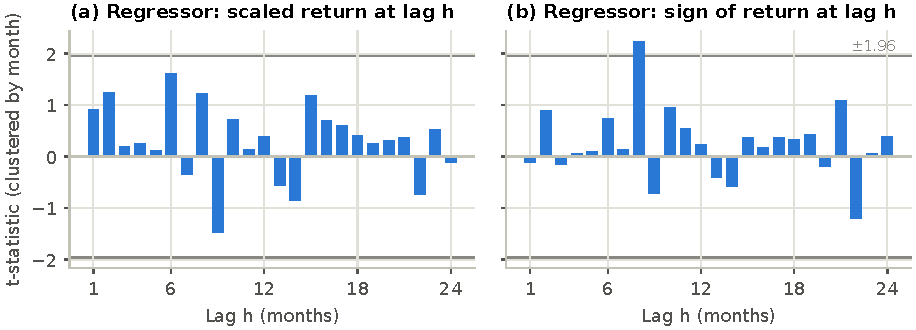
\includegraphics[width=\textwidth]{figures/fig05_predictive_tstats.pdf}
\caption{Pooled regressions of the volatility-scaled return on its own value (a) and sign (b) at lag $h$ months. Horizontal lines mark $\pm 1.96$.}
\label{fig:predictive}
\end{figure}

\end{document}
